\documentclass{article}
\usepackage{amssymb}
\usepackage{amsmath}
\usepackage{graphicx}
\usepackage{epstopdf}

\graphicspath{"C:/Users/Sakshi/Dropbox/IFMR Summit/"}

\begin{document}
	\title{\textbf{\LaTeX - Exercise} \\
	\textbf{\small{\emph{IFMR Summit 2015}}}}
	
	\author{XYZ}
	\maketitle
	
	\begin{center}
	This is an exercise to understand the basic functions of \LaTeX. 
	\end{center}
	
	\newpage
	\tableofcontents
	\newpage
	
	
\section{Equations}
	\begin{enumerate}
		\item \textbf{Single Equation}
			\begin{equation}
			income =  \alpha + \beta_1 . education + \beta_2 . age + \delta . gender\_dummy + \epsilon
			\end{equation}
			
		\item \textbf{Long equation}
			\begin{multline*}
					income =  \alpha + \beta_1 . education + \beta_2 . age + \delta . gender\_dummy\\
					+ \delta_u . urban + \delta_r . rural + \epsilon
			\end{multline*}
			
		\item \textbf{Split environment}
		\begin{equation}
		\begin{split}
			z &= x + x + x + y + y \\
			  &= 3x + 2y
		\end{split}
		\end{equation}
		
		\item \textbf{Align Environment}
		
			\begin{align*}
			 3x + 2y &= 34 \\
			 2x + y  &= 20 
			\end{align*}
	
				\item \textbf{Matrix} \\
				
				\[
				\begin{bmatrix}
					x & y \\
					z & v
				\end{bmatrix}
				\]
				
	\end{enumerate}
	
\section{Tables}
	\begin{tabular}{|c|c|c|}
	\hline Prisoner 1/Prisoner 2 & Confess & Deny \\ 
	\hline Confess & $(-3,-3)$ & $(-1,-5)$ \\ 
	\hline Deny & $(-5,-1)$ & $(0,0)$ \\ 
	\hline 
	\end{tabular} 
	
\newpage	
\section{STATA Output}
	\begin{itemize}
	\item \textbf{Regression output}
		\begin{table}[htbp]\centering
\def\sym#1{\ifmmode^{#1}\else\(^{#1}\)\fi}
\caption{Sample regression}
\begin{tabular}{l*{2}{c}}
\hline\hline
            &\multicolumn{1}{c}{(1)}&\multicolumn{1}{c}{(2)}\\
            &\multicolumn{1}{c}{Without regional dummies}&\multicolumn{1}{c}{Including regional dummies}\\
\hline
lexp        &     -0.0651\sym{**} &     -0.0397         \\
            &     (0.047)         &     (0.103)         \\
[1em]
gnppc       & -0.00000986         & -0.00000286         \\
            &     (0.498)         &     (0.791)         \\
[1em]
1.region    &                     &           0         \\
            &                     &         (.)         \\
[1em]
2.region    &                     &       1.211\sym{***}\\
            &                     &     (0.000)         \\
[1em]
3.region    &                     &       1.297\sym{***}\\
            &                     &     (0.000)         \\
[1em]
\_cons      &       5.768\sym{**} &       3.433\sym{**} \\
            &     (0.012)         &     (0.045)         \\
\hline
\(N\)       &          63         &          63         \\
F           &       6.765         &       19.46         \\
r2          &       0.184         &       0.573         \\
\hline\hline
\multicolumn{3}{l}{\footnotesize \textit{p}-values in parentheses}\\
\multicolumn{3}{l}{\footnotesize This is a sample regression.}\\
\multicolumn{3}{l}{\footnotesize \sym{*} \(p<.10\), \sym{**} \(p<.05\), \sym{***} \(p<.01\)}\\
\end{tabular}
\end{table}

		
	\item \textbf{Data Matrix} \\
		\documentclass[]{article}\pagestyle{empty}\begin{document}
\begin{center}
\begin{tabular}{lcccc}
\hline \noalign{\smallskip} & N. and S. America & Europe and C. Asia & Difference & (p-value)\\
\noalign{\smallskip}\hline \noalign{\smallskip}GNP per capita & 4,829.82 & 10,738.05 & -5,908.23 & 0.03\\
Life expectancy & 70.83 & 73.07 & -2.23 & 0.06\\
(n) & 24.00 & 44.00 &  & \\
\noalign{\smallskip}\hline\end{tabular}\\
\end{center}
\end{document}

		
	\newpage	
	\item \textbf{Graph} \\
	\\
		  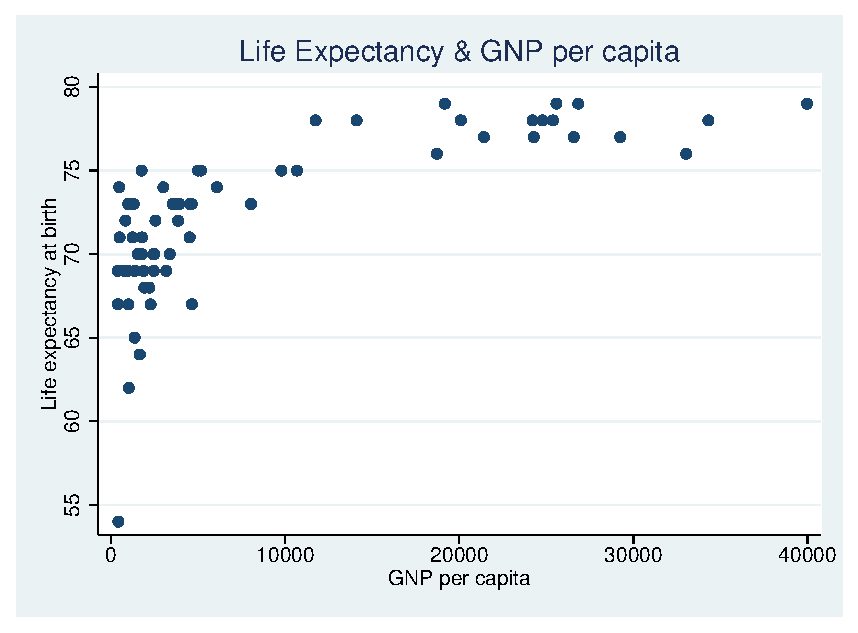
\includegraphics[height=3in]{lexp_gnp1.eps} 	
	
	\end{itemize}
	
	
\end{document}